\documentclass[10pt]{article}
\usepackage[margin=0.78in]{geometry}
\usepackage{graphicx,booktabs,longtable,array,amsmath,amssymb,natbib,microtype,placeins}
\usepackage[hidelinks]{hyperref}
\usepackage[font=small]{caption}
\setlength{\parindent}{0pt}\setlength{\parskip}{4pt}\sloppy
\newcommand{\evidencelabel}[1]{\textbf{#1}\enspace}
\newcommand{\AuthorInputRequired}[1]{\textit{Author input required: #1}}
\title{Confirmatory evaluation separates uncertainty calibration from discovery performance in materials active learning}
\author{Renjie Li\\[2pt]\normalsize Southwest University}
\date{}
\begin{document}\maketitle

\begin{abstract}
Predictive uncertainty has two operational roles in materials active learning:
it supports interval interpretation and it directs acquisition. Whether a
mapping helps one role therefore does not determine its value in the other. We
introduced a role-decomposed confirmatory evaluation that placed uncertainty
transformations in calibration-only, acquisition-only, joint, or
exploration-matched control pathways. Independent confirmation covered four
Matbench regression tasks, two study-defined splits, two bagged-tree models,
and 40 paired seeds in each of 16 environments. Complex global and
candidate-specific mappings did not improve the registered calibration or
top-tail discovery endpoints. A residual-ratio scalar reduced pooled
calibration error, but only 8 of 16 environment estimates had the favorable
direction, limiting transportability. A stagewise exploration control partly
recovered the discovery loss of the original global mapping: pooled recall
nAUC increased from 0.565322 to 0.596941, yet remained below the raw-uncertainty
baseline of 0.641635. A fixed exploration control showed no detectable
difference from the original global mapping; this was not an equivalence test.
The results support role-specific evaluation rather than a universal method
ranking. Their scope is restricted to offline finite pools, composition-only
descriptors, and Random Forest/ExtraTrees uncertainty on four tasks.
\end{abstract}

\section{Introduction}
Finite-budget materials screening is governed by acquisition decisions, not
predictive accuracy alone
\citep{lookman2019active,xue2016adaptive,kusne2020closedloop,rohr2020metrics,hase2021olympus}.
Recent materials benchmarks likewise show that regression quality, uncertainty
quality, and task-relevant discovery metrics need not rank models identically
\citep{varivoda2023uq,riebesell2025matbenchdiscovery}. In an active-learning
campaign, uncertainty informs both the interpretation of predictions and the
choice of the next candidate. Upper-confidence-bound (UCB) acquisition makes
the second role explicit by combining a predictive mean with an
uncertainty-weighted exploration term
\citep{auer2002ucb,srinivas2010gpucb,shahriari2016bo,frazier2018tutorial}.

These roles depend on different properties of the uncertainty signal.
Calibration concerns probabilistic interval behavior; uncertainty ranking
orders candidates; exploration pressure allocates a finite budget; and
trajectory feedback changes later training data. These properties interact,
but they are not interchangeable
\citep{gneiting2007proper,kuleshov2018calibrated,guo2017calibration,angelopoulos2023conformal,mandi2022decision,wilder2019decision,donti2017task}.
A global uncertainty multiplier may change interval widths and the effective
UCB coefficient without changing candidate order. A candidate-specific
mapping can also change the order, which can redirect later training data and
query trajectories.

Most policy benchmarks compare these components jointly. A different query
trajectory can then reflect changed interval scale, changed candidate ranking,
changed effective exploration, trajectory feedback, or several pathways at
once. Such comparisons estimate policy performance but do not localize the
role through which a transformation acts.

We address this identification problem with an operationally role-decomposed
framework: calibration-only, acquisition-only, and joint mappings are compared
with identity and matched-exploration controls
(Fig.~\ref{fig:role-decomposition}). Fixed and stagewise matched-beta controls
isolate exploration pressure without treating it as probabilistic
recalibration. The framework is the contribution; it is neither a new
surrogate model nor a claim of a universally optimal acquisition algorithm.

Development evidence is necessary for strategy construction, but it cannot
serve as independent confirmation. We froze the environment set, strategies,
endpoints, seed blocks, and multiplicity families before confirmation. Four
Matbench regression tasks, two study-defined splits, and two tree ensembles
yielded 16 environments
\citep{dunn2020matbench,ward2018matminer,butler2018mlmaterials}.
Forty disjoint paired seed blocks then tested calibration error and discovery
performance separately.

The resulting confirmation asks which tested transformations change
calibration, acquisition, both, or neither. It retains unfavorable results,
prespecified environment heterogeneity, and descriptive comparisons without
promoting them to new confirmatory claims. Supplementary Table~S11 compares
this role separation and evidence boundary with representative prior work.

\begin{figure}[tbp]
\centering
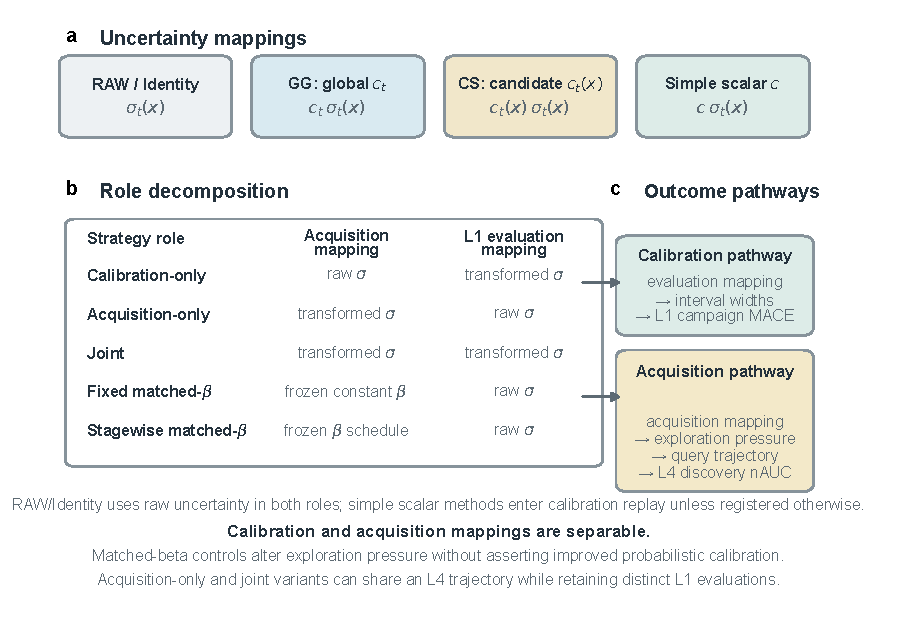
\includegraphics[width=.99\linewidth]{figures_v6/Figure1_uncertainty_role_decomposition.pdf}
\caption{Uncertainty mappings and role-decomposed evaluation. RAW or identity
uses unmodified uncertainty, GG applies a global mapping, CS applies a
candidate-specific mapping, and simple scalar methods apply one calibration
factor. Calibration-only, acquisition-only, and joint variants place the
transformed uncertainty in different campaign roles. The calibration pathway
changes interval widths and L1 campaign MACE. The acquisition pathway changes
exploration pressure, the query trajectory, and L4 discovery nAUC. Fixed and
stagewise matched-beta controls change exploration pressure while retaining
raw uncertainty for evaluation. The schematic contains no effect estimate.}
\label{fig:role-decomposition}
\end{figure}

\section{Methods}

\subsection{Evidence classes, environments, and seed separation}
The V6 confirmation comprised four registered Matbench regression tasks
(\texttt{matbench\_expt\_gap}, \texttt{matbench\_mp\_gap},
\texttt{matbench\_log\_gvrh}, and \texttt{matbench\_log\_kvrh}), two split
types (IID-record and chemical-system-group out-of-distribution), and two
related tree-ensemble models (Random Forest and ExtraTrees). Their Cartesian
product yielded 16 task $\times$ split $\times$ model environments. The
environment set was frozen before confirmation and retained without
post-outcome selection.

Sentinel validation used seeds 6000--6009, and broad development used seeds
6100--6109. Independent confirmation used seeds 7000--7039. Confirmation
trajectories therefore did not enter strategy selection, matched-beta
construction, or policy tuning. Earlier V2, V3, and V5-RC1 stages supplied
exploratory, calibration-evaluation, development, selection, and historical
locked evidence. They document method provenance in Supplementary Fig.~S1 but
were not pooled with V6.

\subsection{Data roles and study-defined splits}
Each task snapshot was partitioned into mutually exclusive source, target, and
diagnostic roles. The source role supplied the seeded initial labelled set.
The target role was the finite candidate pool; a target label entered model
fitting only after that candidate had been queried. The diagnostic role was
never queried and never used to fit the surrogate or an uncertainty mapping;
its labels were read only by checkpoint evaluation. The split validator
required the three roles to be disjoint and exhaustive.

The IID-record split used a seeded permutation with approximately 20\% source,
60\% target, and 20\% diagnostic records. The chemical-system OOD split kept
all compositions with the same sorted element set in one role and assigned
whole groups toward the same proportions. No chemical system crossed roles.
These were study-defined splits over local Matbench task snapshots; the
original Matbench folds were not used.

\subsection{Descriptors and surrogate models}
Formula parsing used pymatgen 2024.10.29 \texttt{Composition}. Each task used
a deterministic, lexicographically ordered elemental atomic-fraction vector
plus total atom count and number of elements: 83 descriptors for experimental
gap and 86 for the other tasks. No feature scaling was applied to surrogate
fitting. The element vocabulary was constructed once over the complete task
without labels, a transductive preprocessing choice that exposes global
element presence but not target values. Random Forest used 80 bootstrap trees, squared-error splits,
unrestricted depth, minimum leaf size two, all features, and one worker
\citep{breiman2001rf,meinshausen2006qrf,wager2014confidence,mentch2016uncertainty}.
ExtraTrees used 80 bootstrap-bagged ExtraTree regressors with random split
thresholds and otherwise matched tree settings
\citep{geurts2006extratrees}. Tree means were averaged; population tree
dispersion was the uncertainty signal, floored at $10^{-8}$. These settings
were common to the compared strategies, so policy differences arose from the
registered uncertainty and acquisition mappings rather than a change of
surrogate class.

\subsection{Campaign geometry and endpoints}
For every task and split, the initial labeled count was
$\max(30,\mathrm{round}(0.01N))$ from the source role; batch size was
$\max(1,\mathrm{round}(0.01N))$; and maximum queries were
$\max(1,\mathrm{round}(0.20N_{\mathrm{target}}))$. Models were retrained after
each simultaneous batch. Ties used descending score and then ascending stable
record index; queried records were removed before rescoring. This deterministic
tie rule ensured that a policy and seed defined one reproducible query
trajectory.

L1 was campaign mean absolute coverage error (MACE), for which lower values
were better. Nominal coverages were 50\%, 80\%, 90\%, and 95\%. At the
initial, 25\%, 50\%, and 75\% campaign checkpoints, MACE was the mean of the
four absolute empirical-minus-nominal coverage errors on the diagnostic role;
the four checkpoint values received equal weight. Gaussian intervals used the
tree mean and effective standard deviation. L1 therefore evaluates the
calibration consequence of an uncertainty mapping along a campaign, rather
than the number of high-value materials found.

L4 was top-1\% recall normalized area under the curve (nAUC), for which higher
values were better. The target set comprised the highest
$\max(1,\lceil0.01N_{\mathrm{target}}\rceil)$ selectable targets, ordered by
target and then stable ID. Recall was integrated against queried-budget
fraction by the trapezoid rule, including the initial state at budget fraction
zero, and divided by the observed x-range. L4 depends on the ordered sequence
of queried candidates and therefore assesses a different consequence of the
policy from L1.

\subsection{Uncertainty transformation and acquisition decomposition}
Let $\mu_t(x)$ and $\sigma_t(x)$ denote the surrogate mean and raw uncertainty
for candidate $x$ at campaign step $t$. The registered raw UCB score was
\begin{equation}
a_{\mathrm{RAW}}(x,t)=\mu_t(x)+\beta\sigma_t(x).
\end{equation}
The Gaussian-global (GG) mapping used a fitted global factor $c_t$,
\begin{equation}
a_{\mathrm{GG}}(x,t)=\mu_t(x)+\beta c_t\sigma_t(x),
\end{equation}
with
\begin{equation}
c_t=\max\!\left(10^{-8},
\frac{\operatorname{median}_{i\in\mathcal O_t}
|y_i-\hat\mu_{i,\mathrm{OOB}}|/
\max(\hat\sigma_{i,\mathrm{OOB}},10^{-8})}
{0.67448975}\right).
\end{equation}
Here $\mathcal O_t$ contains currently labelled records with at least eight
finite OOB predictions. The mapping was refitted after every campaign update;
insufficient OOB support returned identity scaling. Frozen V5-derived GG and
CS policies retain their historical ordered queried-target/OOB pairing for
trajectory identity. New scalar mappings use aligned training-order OOB
targets.

The candidate-specific (CS) mapping used $c_t(x)$,
\begin{equation}
a_{\mathrm{CS}}(x,t)=\mu_t(x)+\beta c_t(x)\sigma_t(x).
\end{equation}
Thus, GG changes the uncertainty scale at a campaign step, while CS can also
change the relative uncertainty contribution across candidates. The selected
CS model uses standardized log raw uncertainty with an intercept. It samples
at most 20,000 unequal-target OOB pairs and minimizes a top-10\%-weighted
pairwise logistic ranking loss plus $0.01$ coefficient and mean-log-scale
penalties. Candidate log scales are clipped to
$[\log(0.25),\log(4)]$; fewer than 30 labelled records or insufficient OOB
support returns the raw policy. The historical CS comparator uses six local
features (raw uncertainty, leaf density, descriptor distance, predictive-mean
percentile, local standardized residual, and local residual dispersion).

For the NLL scalar, aligned OOB residuals $r_i$ determine
\begin{equation}
\hat c_{\mathrm{NLL}}=\arg\min_{0.05\le c\le20}
\frac{1}{|\mathcal O_t|}\sum_{i\in\mathcal O_t}
\left[\log(c\sigma_i)+\frac{r_i^2}{2c^2\sigma_i^2}\right]
=\operatorname{clip}_{[0.05,20]}
\sqrt{\operatorname{mean}(r_i/\sigma_i)^2}.
\end{equation}
The residual-ratio scalar instead uses
$\hat c_{\mathrm{RR}}=\operatorname{clip}_{[0.05,20]}
\{\operatorname{median}(|r_i|/\sigma_i)/0.6744897501960817\}$.
Both use OOB, not held-out diagnostic, residuals; both are refitted each round
and affect calibration evaluation only in their registered comparisons.

The two matched-beta controls retained raw $\sigma_t(x)$ and changed only the
exploration coefficient:
\begin{align}
a_{\mathrm{fixed}}(x,t) &=
\mu_t(x)+\beta_{\mathrm{fixed}}\sigma_t(x),\\
a_{\mathrm{stage}}(x,t) &=
\mu_t(x)+\beta_{s(t)}\sigma_t(x).
\end{align}
For each held-out task, $\beta_{\mathrm{fixed}}$ was the median across
environment-level medians of Original-GG effective beta from the other three
tasks and development seeds 6100--6109. The same leave-one-task-out rule was
applied separately within budget stages $[0,0.25)$, $[0.25,0.50)$,
$[0.50,0.75)$, and $[0.75,1]$ to obtain $\beta_{s(t)}$. The resulting
task-specific constant and schedule were frozen before confirmation; no stage
required fallback. Confirmation outcomes did not enter either value. The
controls consequently test changes in exploration pressure without asserting
that raw probabilistic uncertainty was recalibrated.

The calibration and acquisition roles were assigned independently
(Fig.~\ref{fig:role-decomposition}). Calibration-only strategies acquired with raw
$\sigma$ and evaluated L1 with transformed $\sigma$. Acquisition-only
strategies acquired with transformed $\sigma$ and evaluated L1 with raw
$\sigma$. Joint strategies used transformed $\sigma$ for both operations.
Matched-beta controls acquired with the frozen beta policy and evaluated with
raw $\sigma$. Identity used raw $\sigma$ in both roles. Simple scalar methods
entered calibration replay unless a different role was explicitly registered.

Acquisition-only and joint variants can have identical L4 results because L4
is a functional of the acquisition trajectory. When two variants use the same
acquisition mapping, stable tie rules yield the same ordered queries even if
their L1 evaluation mappings differ. They remain distinct strategies for L1,
where the reported interval widths depend on whether raw or transformed
uncertainty is evaluated.

\subsection{One complete campaign step}
At each step the implementation executed the following fixed sequence:
\begin{enumerate}
\item fit the registered surrogate to all currently labelled source and queried
target records using the deterministic round-specific seed;
\item compute candidate and diagnostic predictive means and raw ensemble
standard deviations;
\item fit the registered mapping from eligible labelled OOB records, or retrieve
the frozen fixed/stagewise beta;
\item construct the registered UCB score and order candidates by descending
score, breaking ties by ascending stable record ID;
\item query the leading batch, reveal only those target labels, and append them
to the labelled set;
\item refit at registered checkpoints, apply the evaluation mapping to the
untouched diagnostic role, and record calibration quantities;
\item update recall against the fixed top-target set and, after the campaign,
compute the registered calibration and discovery endpoints.
\end{enumerate}




\subsection{Strategies and registered comparisons}
The frozen design compared GG and CS calibration-only variants with RAW on L1.
It compared their acquisition-only and joint policies with RAW on L4. Fixed
and stagewise matched-beta controls were compared with Original GG on L4. NLL
and residual-ratio scalar scaling were compared with Identity Control on L1.
Residual-ratio scaling versus the development-selected CS joint policy was
estimation-only, and the cross-endpoint direction table was descriptive.

Original GG denotes the joint GG policy with nominal $\beta=1$, whereas
development-selected GG denotes the historically selected policy with nominal
$\beta=0.5$. Machine identifiers remain unchanged and are mapped to display
names in \path{tables/display_name_mapping.csv}. Acquisition-only and joint
variants can share L4 values because L4 depends on their common acquisition
trajectory. They remain distinct for L1 when their evaluation mappings differ.

\subsection{Locked inference and result control}
Every effect was defined as strategy minus baseline. The pooled inferential
unit was the registered seed block: within each of the 40 shared seeds, the
effect was averaged equally across all 16 environments, and inference was
performed on those 40 paired block effects. The 640 environment-seed
observations were not treated as independent scientific replicates.
Confidence intervals used 10,000 paired bootstrap samples, and confirmatory
p-values used 10,000 paired sign-flip permutations with add-one p-values.
Benjamini--Hochberg correction was applied separately within the four frozen
families. A 40-pair completeness gate was required for every registered
environment; all 176 gates passed.

Task-, split-, model-, and environment-level estimates were retained as
heterogeneity diagnostics and did not replace pooled inference. They were
reported to reveal transportability across the locked environment set, not to
select a favorable subgroup. H6 and H7 were descriptive only. Analysis inputs
were frozen before confirmation outcomes, and the result tables were bound by
\path{locks/v6_p0_confirmation_inference_result_lock.json}. No new
contrast, environment selection, statistical test, or model run was
introduced for this revision.

This statement applies to the locked V6 analysis. A separately prespecified
P1 extension was frozen after V6 and before any P1 outcome. It uses disjoint
sentinel (8000--8004), development (8100--8109), and confirmation
(8200--8239) seeds, and its multiplicity families cannot be pooled with V6.

\subsection{Prespecified P1 extension}
The P1 extension adds a non-bagged conditional-quantile mechanism. A central
gradient-boosting regressor estimates $\mu(x)$, while regressors at quantiles
0.16 and 0.84 estimate $q_{.16}(x)$ and $q_{.84}(x)$. The registered spread is
\begin{equation}
 \sigma_q(x)=\max\left\{\frac{q_{.84}(x)-q_{.16}(x)}
 {2\Phi^{-1}(.84)},10^{-8}\right\}.
\end{equation}
It is an interval-derived conditional predictive-spread proxy, not a
decomposition into epistemic and aleatoric uncertainty. Three role arms share
the same surrogate hyperparameters: raw mapping, residual-ratio
calibration-only, and residual-ratio acquisition-only. Five-fold cross-fitted
labelled residuals fit the scalar; diagnostic targets never fit a mapping.

The P1 endpoint registry adds coverage, width, interval score, Gaussian NLL,
Gaussian-proxy CRPS, standardized-residual and conditional-coverage
diagnostics, along with top-5\%/10\% recall, regret, enrichment, time-to-hit,
random-gain, and budget-segment summaries. Only the prospectively designated
L1 and L4 contrasts are confirmatory. A compute gate requires complete
environment pairs and blocks confirmation when projected wall time exceeds
24 h.

\subsection{Reproducibility and audit trail}
The frozen strategy map records the acquisition and L1 evaluation mapping for
each policy. The endpoint registry fixes direction and aggregation, while the
contrast table fixes the strategy, baseline, and multiplicity family. The
pair-completeness table confirms that all required environments contain the
same 40 confirmation seeds. The inference lock binds pooled effects,
confidence intervals, p-values, and adjusted decisions.

Figures read stored rows directly, and rounding is confined to printed
labels. Supplementary Information provides the full registered results,
environment diagnostics, completeness gates, strategy registry, coefficient
tables, evidence lineage, and source hashes. No historical effect contributes
to a V6 estimate, interval, or p-value.

\section{Results}
\subsection{Locked analysis and reporting conventions}
L1 was lower-is-better campaign MACE, and L4 was higher-is-better top-1\%
recall nAUC. Every effect was strategy minus baseline. Pooled inference used
40 paired seed blocks, each averaging the 16 environments equally.
Confidence intervals used the registered paired bootstrap, and p-values used
the registered paired sign-flip procedure. Benjamini--Hochberg correction was
applied within each frozen family. Environment estimates remained
heterogeneity diagnostics.

\subsection{Complex calibration scaling did not improve calibration error}
GG calibration-only scaling increased L1 relative to RAW (effect, 0.065777;
95\% CI, 0.062782 to 0.068971; adjusted $p=1.000$). The effect was unfavorable
in all 16 environments. CS calibration-only scaling was also unfavorable at
the pooled level (effect, 0.095898; 95\% CI, 0.090827 to 0.100888; adjusted
$p=1.000$), with heterogeneous environment estimates. Values near one reflect
effects opposite to the registered lower-is-better alternative. They do not
show equivalence or absence of an effect.

\begin{figure}[tbp]
\centering
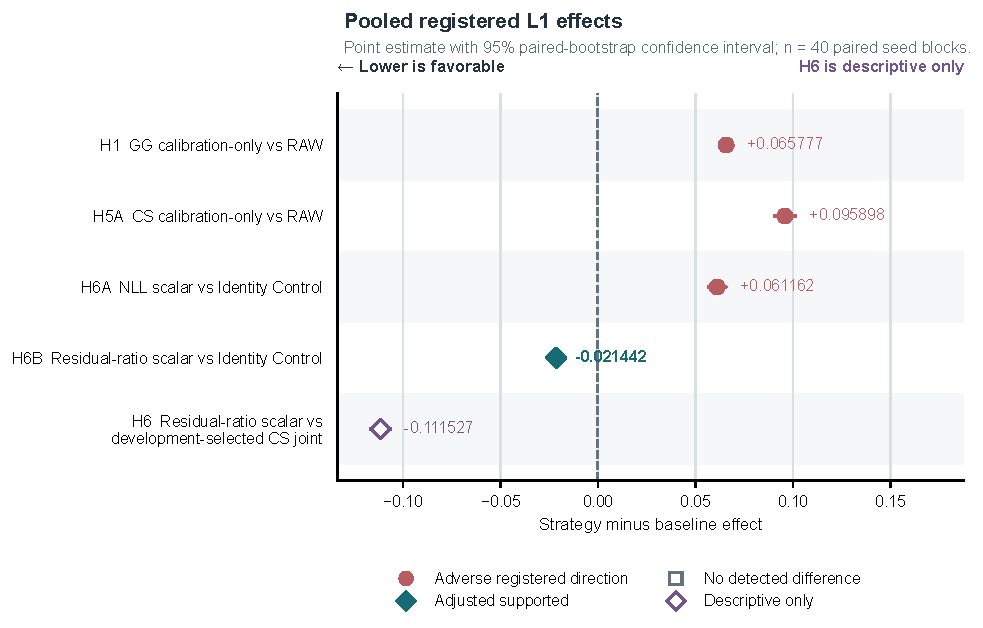
\includegraphics[width=.99\linewidth]{figures_v6/Figure2_L1_pooled_effects.pdf}
\caption{Pooled registered L1 effects. Effects are strategy minus baseline,
and lower values favor the strategy. Points and horizontal lines are locked
pooled effects and 95\% paired-bootstrap confidence intervals. Residual-ratio
scaling versus development-selected CS is descriptive only and has no binary
test. Residual-ratio scaling versus Identity Control remained supported after
family-specific correction, but only 8 of 16 environment estimates shared the
pooled favorable direction.}
\label{fig:l1-pooled}
\end{figure}

\subsection{Complex acquisition and joint scaling did not improve discovery}
GG acquisition-only scaling reduced L4 relative to RAW (effect, -0.076313;
95\% CI, -0.085283 to -0.067686; adjusted $p=1.000$). GG joint, nominal
$\beta=1$, had the same point estimate and a separately resampled 95\% CI of
-0.085393 to -0.067613 (adjusted $p=1.000$). CS acquisition-only scaling and
the development-selected CS joint policy were also unfavorable (both effects,
-0.034084; adjusted $p=1.000$). Their respective 95\% CIs were -0.039446 to
-0.028599 and -0.039606 to -0.028612. Neither complex mapping improved the
registered discovery outcome.

\subsection{Matched-beta controls distinguished fixed and stagewise exploration policies}
Fixed matched-beta showed no detectable L4 difference from Original GG
(effect, -0.000236; 95\% CI, -0.005992 to 0.005446; adjusted $p=0.936$).
This was not an equivalence test and does not establish identity or
interchangeability. Stagewise matched-beta increased L4 relative to Original
GG (effect, 0.031619; 95\% CI, 0.025535 to 0.037613; adjusted $p<0.001$).
All 16 environment estimates were favorable. The comparison identifies a
performance difference, not a unique causal mechanism.

Absolute pooled levels provide the necessary baseline: RAW was 0.641635,
Original GG was 0.565322, and stagewise matched-beta was 0.596941. Thus the
registered stagewise-minus-Original-GG effect was $+0.031619$, while the
stagewise-minus-RAW difference was $-0.044694$. The latter comparison is
descriptive, was not registered for a confirmatory p-value, and was not added
to a multiplicity family. Stagewise matched-beta therefore partly recovered
the discovery loss of Original GG but did not establish superiority or
noninferiority to RAW. Original GG is the H4 baseline because the earliest
registry named its alias, GG joint; the matched-beta control was designed to
isolate Original GG's effective exploration pressure, not to test overall
performance against RAW.

\begin{figure}[tbp]
\centering
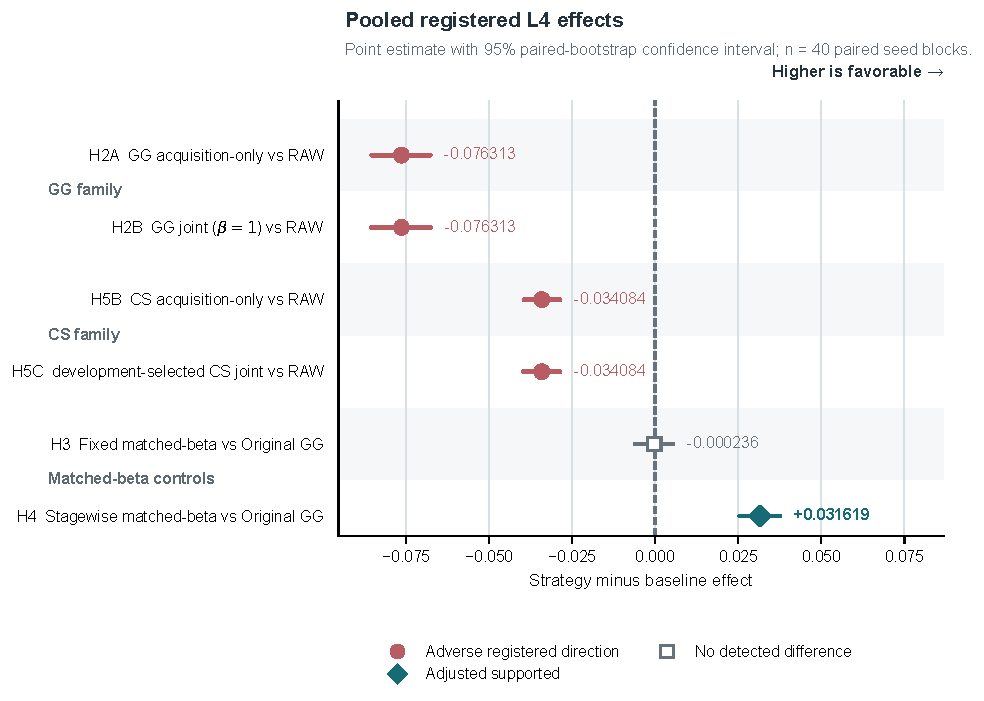
\includegraphics[width=.99\linewidth]{figures_v6/Figure3_L4_pooled_effects.pdf}
\caption{Pooled registered L4 effects. Effects are strategy minus baseline,
and higher values favor the strategy. Points and horizontal lines are locked
pooled effects and 95\% paired-bootstrap confidence intervals. Fixed
matched-beta showed no detectable difference and was not an equivalence test.
Stagewise matched-beta was the adjusted positive L4 finding. Acquisition-only
and joint GG or CS pairs share point estimates because each pair generated the
same acquisition trajectory.}
\label{fig:l4-pooled}
\end{figure}

\subsection{Simple scalar scaling showed method-specific and heterogeneous calibration effects}
NLL scalar scaling increased L1 relative to Identity Control (effect,
0.061162; 95\% CI, 0.056963 to 0.065341; adjusted $p=1.000$).
Residual-ratio scalar scaling reduced pooled L1 (effect, -0.021442; 95\% CI,
-0.023667 to -0.019147; adjusted $p<0.001$). Only 8 of 16 environment
estimates shared the favorable direction, with effects ranging from -0.064399
to 0.019515. The pooled improvement therefore did not establish uniform
transportability. The corresponding absolute pooled levels were 0.069511 for
Identity Control and 0.048069 for residual-ratio scaling.

Residual-ratio scaling also had lower L1 than the development-selected CS
joint policy (effect, -0.111527; 95\% CI, -0.116235 to -0.106876). All 16
environment estimates were negative. This comparison was descriptive only and
had no binary test or multiplicity assignment. It does not establish
superiority or noninferiority.

\subsection{Environment heterogeneity and completeness}
Environment diagnostics qualified the pooled results without replacing them.
Stagewise matched-beta was favorable in 16 of 16 environments. The pooled
residual-ratio improvement was favorable in 8 of 16 environments. All
registered comparisons satisfied the 40-pair completeness requirement.

\begin{figure}[tbp]
\centering
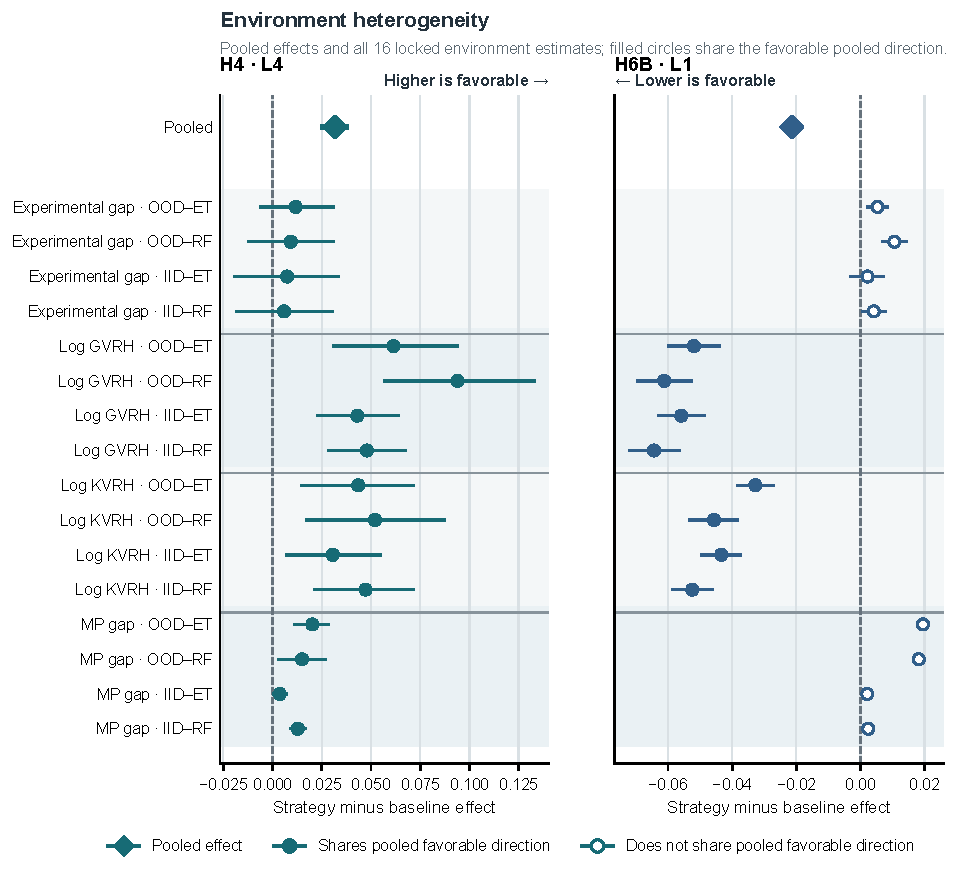
\includegraphics[width=.99\linewidth]{figures_v6/Figure4_H4_H6B_environment_heterogeneity.pdf}
\caption{Environment heterogeneity for stagewise matched-beta and
residual-ratio scaling. Points and horizontal lines are locked environment
effects and 95\% paired-bootstrap intervals, grouped by task. Stagewise
matched-beta was favorable in 16 of 16 environments, whereas residual-ratio
scaling was favorable in 8 of 16. These diagnostics qualify but do not replace
pooled inference.}
\label{fig:heterogeneity}
\end{figure}

\subsection{Complete registered-result summary}
Table~\ref{tab:registered-summary} reports every registered pooled comparison.
The full-precision table, multiplicity families, and H7 descriptive direction
table are provided in Supplementary Information.

\FloatBarrier
\begin{table}[!tbp]
\centering
\caption{Condensed V6 registered-result summary. Effects are strategy minus
baseline. L1 is lower-is-better and L4 is higher-is-better. The p-value column
reports the registered BH-adjusted result.}
\label{tab:registered-summary}
\scriptsize
\begin{tabular}{llrrrrl}
\toprule
ID & Endpoint & Effect & CI low & CI high & Adjusted $p$ & Interpretation\\
\midrule
H1  & L1 &  0.065777 &  0.062782 &  0.068971 & 1.000 & Unfavorable\\
H5A & L1 &  0.095898 &  0.090827 &  0.100888 & 1.000 & Unfavorable, heterogeneous\\
H2A & L4 & -0.076313 & -0.085283 & -0.067686 & 1.000 & Unfavorable\\
H2B & L4 & -0.076313 & -0.085393 & -0.067613 & 1.000 & Unfavorable\\
H5B & L4 & -0.034084 & -0.039446 & -0.028599 & 1.000 & Unfavorable, 16/16\\
H5C & L4 & -0.034084 & -0.039606 & -0.028612 & 1.000 & Unfavorable, 16/16\\
H3  & L4 & -0.000236 & -0.005992 &  0.005446 & 0.936 & No detectable difference\\
H4  & L4 &  0.031619 &  0.025535 &  0.037613 & $<0.001$ & Supported, 16/16\\
H6A & L1 &  0.061162 &  0.056963 &  0.065341 & 1.000 & Unfavorable\\
H6B & L1 & -0.021442 & -0.023667 & -0.019147 & $<0.001$ & Supported, heterogeneous\\
H6  & L1 & -0.111527 & -0.116235 & -0.106876 & -- & Descriptive only\\
\bottomrule
\end{tabular}
\begin{minipage}{.98\linewidth}\footnotesize\smallskip
One-sided BH-adjusted p-value refers to registered favorable-direction tests;
H3 and H4 retain their registered two-sided matched-beta tests. Tests targeted
the prospectively registered favorable direction. Effects lying in the
opposite direction therefore yield one-sided p-values near 1; such values do
not indicate equivalence or absence of an effect. H6 had no binary test or
multiplicity assignment.
\end{minipage}
\end{table}

\subsection{P1 implementation and compute-gate status}
The prespecified P1 model, metric, checkpoint, retry, and manifest code passed
implementation tests. Real-data sentinels used only seeds 8000--8004, and a
bounded exploratory development audit used 8100--8109. These runs validate
execution and measure cost; they are not confirmation evidence. The full
3,520-job candidate manifest was projected to require 48--55 h with two
workers, so the registered 24-h gate stopped execution before seeds
8200--8239. Accordingly, no P1 pooled effect, confidence interval, p-value, or
claim is reported here. Supplementary Section S12 records the diagnostic
figures and their evidence classes.

\begin{table}[!tbp]
\centering
\caption{Condensed V6 claim-evidence classification. H7 is an analysis-only
direction table, and H6 is an estimation-only comparison.}
\label{tab:claim-classification}
\small
\begin{tabular}{lll}
\toprule
Claim class & Hypotheses & Evidence-constrained conclusion\\
\midrule
Adjusted confirmation & H4, H6B & Positive pooled findings; H6B heterogeneous\\
Contradicted direction & H1, H5A, H2A, H2B, H5B, H5C, H6A & Improvement not supported\\
No detected difference & H3 & Near-zero mean; no equivalence test\\
Descriptive only & H6, H7 & No binary, superiority, or causal claim\\
\bottomrule
\end{tabular}
\end{table}
\FloatBarrier

\section{Discussion}
\subsection{Calibration and discovery are separate evaluation targets}
Calibration-only, acquisition-only, and joint variants provide a reusable
design pattern for identifying where an uncertainty transformation enters an
active-learning campaign. L1 evaluates interval behavior along the campaign,
whereas L4 evaluates top-tail discovery along the query trajectory. Neither
endpoint can substitute for the other. The design does not assume that the
roles are causally independent; it makes their operational placement explicit.

This distinction is useful because a global scale can change interval widths
and effective exploration pressure without changing the ordering induced by
raw uncertainty itself: with UCB, multiplying every uncertainty by $c_t$ is
algebraically equivalent to replacing $\beta$ by $\beta c_t$. The combined
score can nevertheless reorder candidates relative to another beta because
the balance between mean and uncertainty changes. A candidate-specific
$c_t(x)$ additionally changes uncertainty ranking directly. Reporting only a
joint policy leaves calibration, ranking, exploration, and trajectory feedback
unresolved, even when the policy is operationally convenient.

\subsection{What the unfavorable GG and CS confirmation results establish and do not establish}
The registered GG and CS variants did not improve their corresponding V6
calibration or discovery outcomes. Several pooled intervals lay wholly in the
unfavorable direction. These findings narrow the claim that added mapping
complexity provides a general benefit in the tested settings.

The results do not show that GG or CS is universally invalid. They do not
identify an implementation failure or a single mechanism for the unfavorable
directions. Scaling, ranking, exploration pressure, and trajectory feedback
remain plausible contributors that require separately designed studies.

\subsection{What matched-beta controls reveal about exploration pressure}
Fixed matched-beta showed no detectable difference from Original GG, but the
design did not test equivalence. Stagewise matched-beta was favorable relative
to Original GG across all 16 environments. It partly recovered Original GG's
discovery loss, but its pooled L4 remained 0.044694 below RAW. H4 therefore
establishes a difference from its mechanistic baseline, not overall benefit
relative to the raw policy.

The comparison does not identify a unique mechanism. A stage schedule may
alter when exploration pressure is applied, but that explanation remains a
hypothesis. Mechanism-focused validation would need to vary schedule shape
while holding the other policy components fixed.

\subsection{Scalar calibration gains and environmental heterogeneity}
The simple scalar results show why calibration methods should be named rather
than grouped under a single scaling label. NLL fitting and residual-ratio
fitting optimize different summaries of predictive error and uncertainty.
Only residual-ratio scaling improved the registered pooled L1 comparison.

That pooled gain was favorable in only 8 of 16 environments. This split
direction pattern limits claims of transportability across task, split, and
model settings without invalidating the locked pooled result. The comparison
with development-selected CS was favorable at the descriptive level, but it
had no binary test or multiplicity assignment.

\subsection{Scope, limitations, and future validation}
Locked V6 model and domain scope are limited to four Matbench tasks,
composition-only descriptors, and Random Forest and ExtraTrees. The
prespecified quantile-boosting extension passed implementation and reduced
development checks but did not pass through full independent confirmation;
neural, kernel, and deep-ensemble uncertainty models were not tested. The environment set provides
structured heterogeneity, not universal external validity.

Mechanistic scope is also limited. The study did not causally decompose
scaling, ranking, exploration pressure, and trajectory feedback. The
stagewise matched-beta result identifies a performance difference, not a
unique mechanism. The present results do not establish a universal causal
trade-off between calibration and discovery.

Deployment scope is limited to offline finite-pool benchmarks. The design did
not represent experimental cost, delay, batch failure, synthesis feasibility,
or laboratory validation. L1 and L4 answer the registered questions but do not
form a complete deployment utility function.

Future work should retain independent confirmation, separate calibration and
discovery endpoints, and prespecified environment diagnostics. Studies that
seek a mechanism should manipulate policy components directly and register the
relevant contrasts before outcomes are observed.

\section{Conclusion}
Role-decomposed confirmation separated uncertainty calibration from discovery
performance without changing the underlying campaign evidence. Complex GG and
CS scaling did not improve their registered outcomes in the tested settings.
Stagewise matched-beta partly recovered the discovery loss of Original GG but
remained below RAW, while residual-ratio scaling reduced pooled calibration
error with substantial environment heterogeneity.

Materials active-learning studies should report calibration and discovery
separately and include controls that distinguish uncertainty scaling from
changes in exploration pressure. These conclusions apply only to the tested
implementations on four Matbench task snapshots, study-defined IID and
chemical-system OOD splits, composition-only descriptors, Random
Forest/ExtraTrees surrogates, and offline finite-pool campaigns. They do not
imply a universal method ranking or laboratory-deployment performance.

\section*{Data availability}
The Matbench inputs are publicly obtainable from their original source.
Processed manifests, locked result tables, execution inventories, and
source-binding records are retained in the verified internal package. Public
repository and archive details remain pending author confirmation and are
listed in \path{SUBMISSION_METADATA_TODO.md}.

\section*{Code availability}
The internal package contains the campaign, replay, inference, figure, and
validation code used to reproduce the frozen outputs. A public repository,
archive DOI, and code license must be confirmed before submission; no public
release is claimed here.

\section*{Reproducibility statement}
The frozen V6 strategy map, endpoint registry, raw-result lock,
inference-result lock, registered contrast tables, environment estimates, and
figure source records were checked together. The separate P1 protocol and
implementation locks bind its reduced sentinel/development artifacts. P1 was
not pooled with V6, and no P1 confirmation outcome was generated.

\section*{Author contributions}
\AuthorInputRequired{confirm the proposed CRediT roles listed in
\path{AUTHOR_INPUT_REQUIRED.md}.}

\section*{Competing interests}
\AuthorInputRequired{provide the final competing-interests declaration.}

\section*{Acknowledgements and funding}
\AuthorInputRequired{provide funding and acknowledgement statements, including
grant identifiers where applicable.}

\bibliographystyle{plainnat}
\bibliography{references_submission_candidate_v4_final_r1}
\end{document}
